\chapter{Objetivos y motivación}


\bigskip
Un algoritmo es una serie de pasos organizados que describe el proceso que se debe seguir, para dar solución a un problema específico. A principios de la década de 1960, en 1962 John Henry Holland ideó una de las líneas más prometedoras de la inteligencia artificial, la de los algoritmos genéticos, y con su libro "Adaptation in Natural and Artificial Systems" en 1975 logró una mayor popularidad. 

Son llamados así porque se inspiran en la evolución biológica y su base genético-molecular. Estos algoritmos hacen evolucionar una población de individuos sometiéndola a acciones aleatorias semejantes a las que actúan en la evolución biológica (mutaciones y recombinaciones genéticas), así como también a una selección de acuerdo con algún criterio, en función del cual se decide cuáles son los individuos más adaptados, que sobreviven, y cuáles los menos aptos, que son descartados.

\bigskip
Para su funcionamiento (el de un algoritmo genético simple, llamado Canónico), al empezar necesita una codificación o representación del problema que se adecue al mismo y una función de ajuste o adaptación al problema. Durante la ejecución del algoritmo, los padres deben ser seleccionados para la reproducción, a continuación dichos padres seleccionados se cruzarán generando dos hijos, sobre cada uno de los cuales actuará un operador de mutación. El resultado de la combinación de las anteriores funciones será un conjunto de individuos (posibles soluciones al problema), los cuales en la evolución del algoritmo genético formarán parte de la siguiente población.

\bigskip
Poseen multitud de aplicaciones, como pueden ser:

\begin{itemize}
	\item Diseño automatizado para la investigación de diseño de materiales, equipamiento industrial o sistemas de comercio en el sector financiero.
	\item Construcción de árboles filogenéticos.
	\item Diseño de sistemas de distribución de aguas.
	\item Resolución de equilibrios en Teoría de juegos.
	\item Análisis de expresión de genes.
\end{itemize}

\bigskip
Pueden resolver problemas de alta complejidad, pero esto suele traducirse en operaciones muy costosas en términos de tiempo y recursos. En la actualidad, por ejemplo, hay casos en los que recrear una simulación de la solución propuesta por una iteración puede durar varios días y consumir gran cantidad de procesamiento y recursos asociados.





\bigskip
\section{Objetivos}
\bigskip


\begin{itemize}
	
	\item Se desarrollarán varias clases para lanzar algoritmos genéticos que aprovechen el cálculo paralelo de alguna arquitectura de cálculo especializada (más adelante se vera que se opta por CUDA)
	
	\item Además se desarrollará un servicio web que interactúe con ellas. Esa infraestructura que da soporte a las llamadas del servicio debe hacer uso de una GPU. Esto hará que dichos algoritmos genéticos sean más accesibles y fáciles de usar, ya que sólo tendrán que introducir los parámetros que se deseen y lanzar el algoritmo de manera intuitiva y sin necesidad de una preparación previa.
	
	\item Y se estudiará la posibilidad de publicar dicho servicio para que sea accesible por cualquier usuario de Internet, dependiendo del rendimiento obtenido.
	
\end{itemize}



\bigskip
\section{Motivación}
\bigskip

Dicha complejidad en la resolución de los algoritmos genéticos nos lleva a optimizarlos y a trabajar con ellos para lograr reducir el coste de dichas operaciones. 

Esto nos lleva a utilizar una computación paralela, en la que se aprovecha la potencia de computación de los sistemas con los que trabajamos realizando cálculos simultáneamente. Sigue el principio de dividir los problemas grandes en problemas más pequeños, que se solucionan en paralelo para luego obtener la solución del problema inicial.

Por otra parte, en el ámbito de la computación se ha visto una gran evolución de las tarjetas gráficas, ya que grandes fabricantes como NVIDIA, AMD, IBM o Intel han logrado una producción de GPUs de gran alcance, como se puede ver en la Figura \ref{fig:gpu_vs_cpu} (pueden incluso superar la frecuencia de reloj de una CPU antigua).

\bigskip
\begin{figure}[h]
	\centering
	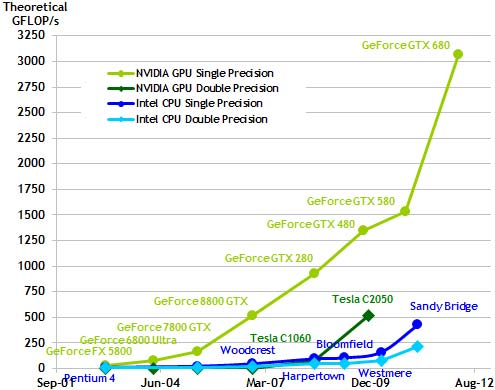
\includegraphics[width=0.7\linewidth]{../images/gpu_vs_cpu}
	\caption[Evolución de las GPUs respecto a las CPUs]{Evolución hasta 2012 de las GPUs respecto a las CPUs}
	\label{fig:gpu_vs_cpu}
\end{figure}


\bigskip
El uso de computación paralela, junto la potencia y la posibilidad de usar el paralelismo que ofrecen las GPU  hace muy interesante el uso de dichas GPUs para resolver algoritmos genéticos de formas más eficiente.

Después del estudio realizado en el siguiente capítulo, se opta por usar la arquitectura de cálculo CUDA \cite{nvidiacuda} para crear algoritmos genéticos que se ejecuten en GPUs de NVIDIA \cite{nvidiadeveloper}.

Como se cita en uno de los objetivos, se publicará de manera que cualquier usuario tenga acceso. Esto, junto a una interfaz sencilla, permitirá computar algoritmos genéticos con facilidad y rapidez.




